\documentclass[fleqn,10pt]{wlscirep}
\usepackage[utf8]{inputenc}
\usepackage{hyperref}
\usepackage[T1]{fontenc}
\usepackage{pdfpages}
\title{Title: G13ODI}
\author{Shubham Bhandari shubhambhandari13@gmail.com}
\affil[]{This is project report for the subject 'CS1305: Business Intelligence' at JK Lakshmipat University, Jaipur}

\begin{abstract}
Cricket is a facinating and a very popular game. There have been many analysis conducted on this game.
This project is about analysing a sample of International One Day matches and also predict the runs scored by Virat Kohli. I have analysed certain hypothesis by
preparing their statistical models in the project. The sample has a scorecard of roughly 1700 ODI matches. The crude data is ball-by-ball performance of player
in these matches which is then subjected to data processing to obtain the scorecard of these matches. 
The descriptive analysis of this data provide some insights in the ODI matches.
This data is then subjectd to t-test statistical model which concludes that the mean wickets fallen in the first 35.3 overs of the first inning is equal to
the wickets fallen in the last 25.3 overs. 
In the end the runs scored by one of the best batsman in ODI have been predicted using linear regression.
\end{abstract}

\begin{document}
\flushbottom
\maketitle
\thispagestyle{empty}
\section{Introduction}
Cricket is one of the most popular game in the world. This project analysis ODI matches dataset and propose some hypothesis.
The hypothesis considered in the project is about the dismissals in the game of the cricket. This project also tries and predict
the runs score by one batsman. The dataset lacks the data of all the players that played in a match which would have result to 
better analysis.
\section{Background}
\subsection{The Game of Cricket}
'Cricket' also known as 'Gentlemen's game' is a bat and ball team sport played between two teams of eleven players each. 
The game is played on a ground at the centre of which is a 22-yard pitch with three wooden stumps at both the ends known as wickets.
The wickets has also has two bails balanced on them. The game has fixed pitch size and variable ground size. 
One of the team act as a batting side in what is called as a inning while the other team at the same time act as the bowline or fielding side.
The batting side score runs by striking the ball bowled to them using bat, and the fielding side tries to catch and stop the ball. 
Team scoring more runs in the specified balls wins the game.
The possible scoring options in cricket include runs ranging from one to six and the possible dissmisal options include clean bowled, run out, caught, leg before wickets
and stumped.
The fielding side tries to restrict the batting side to minimum runs by taking wickets and exhausting the specified balls. 
A cluster of six such balls is known as an over.
The batting side always plays in pair, in which one of the batsman known as striker stands at the further side of the pitch to the bowler and other known as non striker
stand near the bowler.When ten players have been dismissed, the innings ends and the teams swap roles. The game has three umpires, two on the ground and one in a room
with the ability of giving decision with the help of cameras. There is also a match refree in a cricket match.

The game has three popular formats the Twenety20, the One Day International and Test comprising of 20, 50 and unlimited overs respectiverly. Test matches are played for a
duration of five days, where each team gets batting twice.
The ball is a hard, solid spheroid made of compressed leather with a slightly raised sewn seam enclosing a cork core which is layered with tightly wound string. The bat is a
piece of wooden crafted for hitting the ball. The size of bat has some restrictions, exact size depends on the comfort of the player.

Cricket's origins are uncertain, but the earlies reference is in South-East England in the middle of 16th century. Cricket is a highly popular sport 
in the British Colonies.

\subsection{The Cricket Dataset}
The dataset has been obtained from cricsheet.org. The data has ball by ball data of nearly 4000 matches played
between 2006-2019. This data has been then processed to create scorecard file and match information file.
We are using 1,788 ODI matches dataset for this project. The dataset provides various parameters for each match divided in two files.
Match information file comprises of 1788 rows and 25 columns and the scorcard file has 37,963 rows and 23 columns.
This dataset comprises of parameters such as match date, venue umpire, winner, winning runs/wickets etc alongwith scorecard of each match.
The scorecard provides each player's performance in every match. The players who have contributed either through bowling or batting have been included in the dataset.

\subsection{Cricket Betting}
Cricket betting works in two ways, first one is to bet on the outcome of the match and the other one is betting on the outcome of six-overs.
In the case of six-over betting, bets are placed on how many runs can be scored by a team. 
In betting one needs to  analyse the situation and make an educated guess about the outcome and earn money from it. 
In a cricket match, there are several factors that are considered before betting, these factors include weather,pitch report,team combination,strengths and weakness of players,spin and pace combination,past records,player form etc. 
Betting is all mathematics. The ratios or odds offered depend on the situation of the match at a particular instance and the amount of money put on that team.
\subsection{Statistical Models}
Paired Sample T-Test: 
The paired sample t-test, sometimes called the dependent sample t-test, is a statistical procedure used to 
determine whether the mean difference between two sets of observations is zero. In a paired sample t-test, 
each subject or entity is measured twice, resulting in pairs of observations. Common applications of the 
paired sample t-test include case-control studies or repeated-measures designs. Suppose you are interested in 
evaluating the effectiveness of a company training program. One approach you might consider would be to measure 
the performance of a sample of employees before and after completing the program, and analyze the differences 
using a paired sample t-test.

\subsection{Machine Learning Models}
In statistics, linear regression is a linear approach to modeling the relationship between a scalar response (or dependent variable) and one or more explanatory variables (or independent variables). 
The case of one explanatory variable is called simple linear regression. For more than one explanatory variable, the process is called multiple linear regression.This term is distinct from multivariate linear regression, where multiple correlated dependent variables are predicted, rather than a single scalar variable.
In linear regression, the relationships are modeled using linear predictor functions whose unknown model parameters are estimated from the data. Such models are called linear models. Most commonly, the conditional mean of the response given 
the values of the explanatory variables (or predictors) is assumed to be an affine function of those values; less commonly, the conditional median or some other quantile is used. Like all forms of regression analysis, linear regression focuses 
on the conditional probability distribution of the response given the values of the predictors, rather than on the joint probability distribution of all of these variables, which is the domain of multivariate analysis.
\section{Past Work/Related work/Motivation}
With the onset of the era of data and better computing systems, data from practically any field can be used for analysis and 
improve the performance or increase the efficiency of humans in that field. Similarly several studies have already been conducted to prove some popular 
hypothesis or analyse performance of the players. These analysis can actively predict the rising star in the field of cricket or can predict the 
future performance of a player. Such studies also act as an aid for team selection procedure by creating mathematical models for selection of players.
These models can also help us in fantasy cricket.
On similar lines we are trying to dismissal method in a match by away team which can again come handy in fantasy cricket and also team selection for a match.
\section{Evaluation}
\subsection{Methodology}
\subsubsection{Objective of this work}
The objective is to read the provided dataset and analyse the dismissal methods and dismissals of the players.
\subsubsection{Followed Methodology}
\begin{itemize}
    \item Identified the objective and prepared scorecard and match information files accordingly.
    \item Descriptive Analysis of the thus generated data.
    \item Statistical Analysis of the data.
    \item Either accept the null hypothesis or suggest alternate hypothesis also predict the future outcome.
\end{itemize}
\subsection{Descriptive Data Analysis}
The dataset comprises of 1,788 ODI matches data collected from the ODI match held between 03/01/2006-11/7/2019 around the globe. 
The dataset describes player wise statistics of each match. This data is further accumulated to find out the 
method of dismissal method of the player by away team. 
The dataset also has each match's essential data including its venue, city, umpires, teams etc.
The interactive visualizations cannot be shown in LaTex therefore, here is the link for all the Jupyter notebook: \href{https://nbviewer.jupyter.org/github/dev-SB/cricket-bi/blob/master/vis-cricket.ipynb}{vis-cricket.ipynb}.

\begin{itemize}
    \item According to the figure~\ref{fig:one} KC Sangakara is the batsman who has scored most runs and played most balls in the period of Jan 2006-July 2019.
    \begin{figure}[!htb]
        \centering
        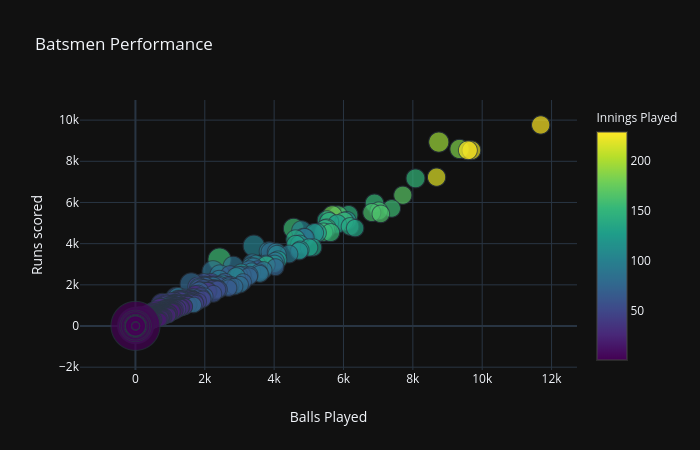
\includegraphics[width=0.6\textwidth]{bats.png}
        \caption{Batsmen performance analysis based on runs scored, balls played and innings played}
        \label{fig:one}
      \end{figure}
      \item According to the Figure ~\ref{fig:two} KC Sangakara was the highest run scorer in 2006 and Rohit Sharma in in 2019(till July)
      \begin{figure}[!htb]
        \centering
        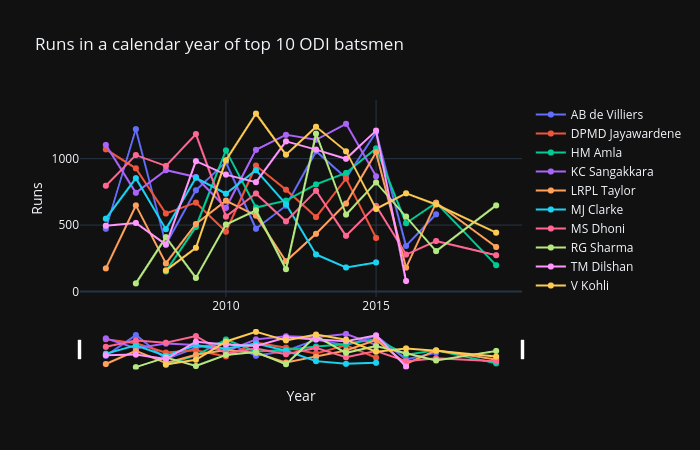
\includegraphics[width=0.6\textwidth]{batsmen.png}
        \caption{Runs in calendar year by top 10 batsmen in ODI}
        \label{fig:two}
      \end{figure}
      \item According to Figure ~\ref{fig:three} all the grounds have nearly 7 wickets fallen in every match.
      \begin{figure}[!htb]
        \centering
        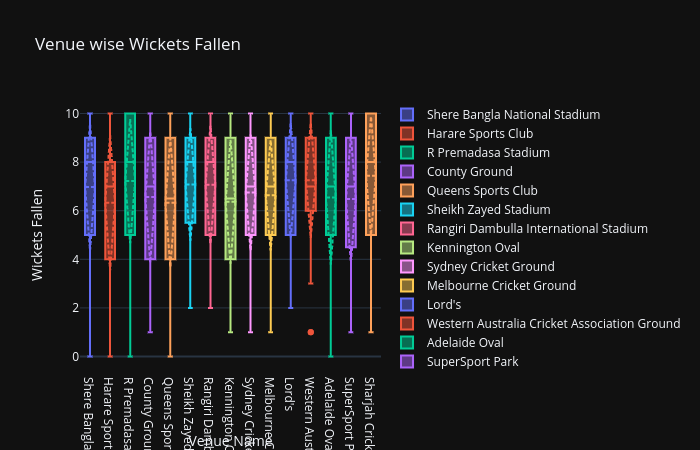
\includegraphics[width=0.6\textwidth]{wicvenue.png}
        \caption{Venue wise wickets fallen.}
        \label{fig:three}
      \end{figure}
      \item According to Figure ~\ref{fig:four} many teams have perfect trackrecord in certain grounds and some teams didn't manage to win even a single match in some grounds.
      \begin{figure}[h]
        \centering
        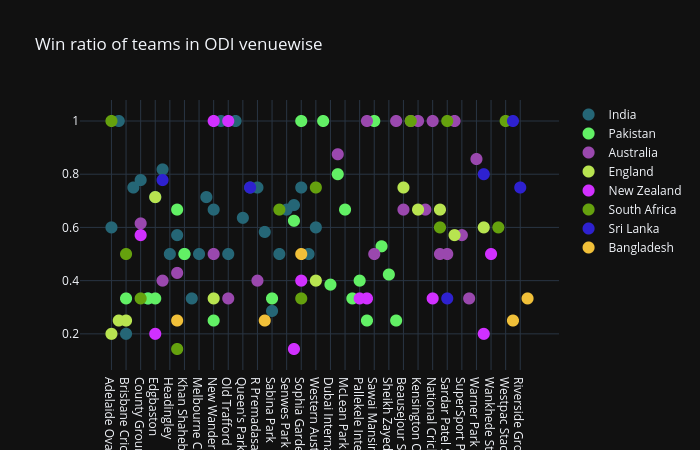
\includegraphics[width=0.6\textwidth]{teamvenue.png}
        \caption{Win ratio of best performing teams venue wise in ODI.}
        \label{fig:four}
      \end{figure}
      
      \item According to Figure ~\ref{fig:five}, Australia was the best team in ODI in 2006 and they have been replaced by India in 2019 (till July).
      \begin{figure}[h]
        \centering
        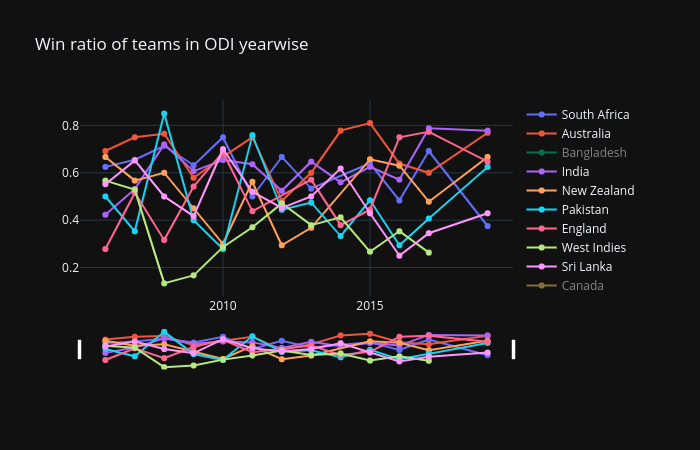
\includegraphics[width=0.6\textwidth]{winteams.png}
        \caption{Win ratio of best performing teams yearwise in ODI}
        \label{fig:five}
      \end{figure}
      \item According to the Figure ~\ref{fig:six}, the median and mean runs scored within the period of 1/2006 and 7/2019 is highest in Sydney Cricket Ground.
      \begin{figure}[h]
        \centering
        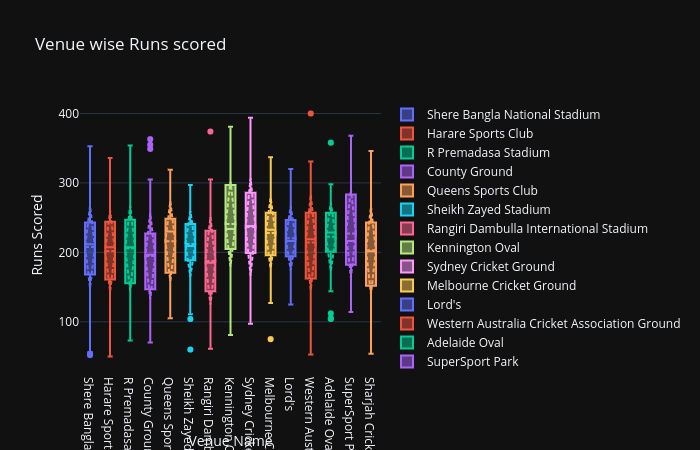
\includegraphics[width=0.6\textwidth]{venueruns.png}
        \caption{Venue wise runs scored.}
        \label{fig:six}
      \end{figure}
      \item According to Figure ~\ref{fig:seven}, Mashrafe Mortaza was the best bowler in 2006 and have been replace by Malinga (The figure only includes top 10 wicket takers in the period of 1/2006-7/2019)
      \begin{figure}[h]
        \centering
        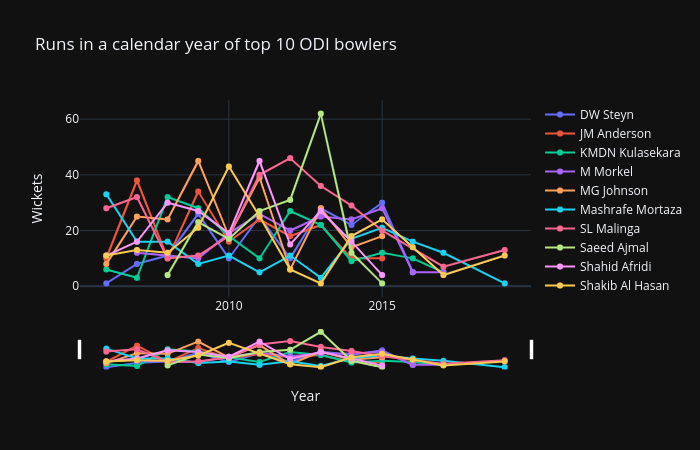
\includegraphics[width=0.6\textwidth]{wicbowlers.png}
        \caption{Wickets in a calendar year by top 10 ODI bowlers.}
        \label{fig:seven}
      \end{figure}
      \item According to Figure ~\ref{fig:eight}, West Indies gives most extras with the mean extras given equal to 8.18 among the prominent cricket playing nations.
      \begin{figure}[h]
        \centering
        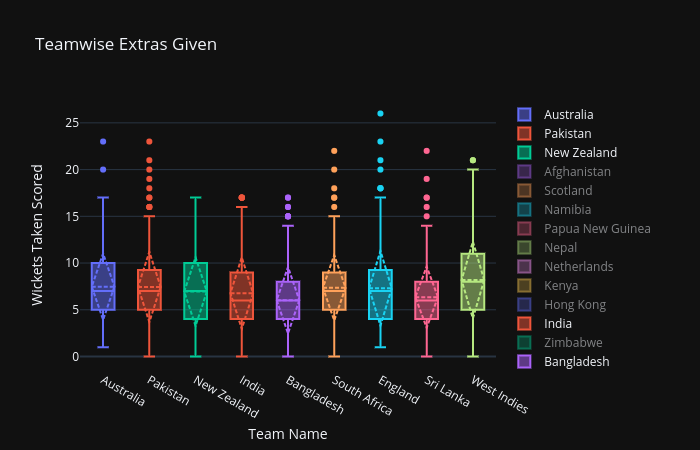
\includegraphics[width=0.6\textwidth]{teamextras.png}
        \caption{Teamwise extras given. }
        \label{fig:eight}
      \end{figure}
      \item According to Figure ~\ref{fig:nine},Australia is the higest runs scorer in every match with the mean of 235 and median 238, closely followed by team India.
      \begin{figure}[h]
        \centering
        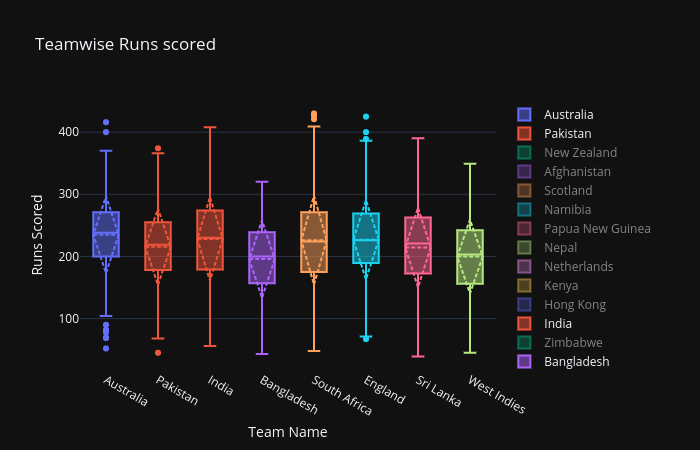
\includegraphics[width=0.6\textwidth]{teamruns.png}
        \caption{Teamwise runs scored.}
        \label{fig:nine}
      \end{figure}
      \item According to Figure ~\ref{fig:ten}, Australia has taken the most number of average wickets per match.
      \begin{figure}[h]
        \centering
        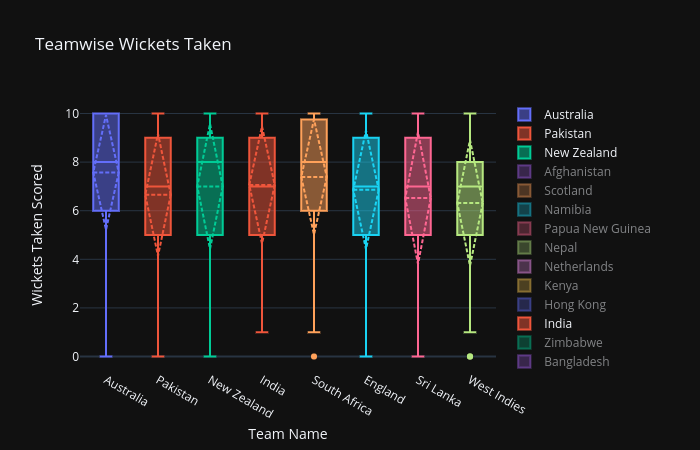
\includegraphics[width=0.6\textwidth]{teamwic.png}
        \caption{Teamwise wickets taken.}
        \label{fig:ten}
      \end{figure}
      

\end{itemize}
\subsection{Statistical Modelling}
Paried sample T-test model has been developed for the statistical analysis of the project. 
\begin{enumerate}
\item
\begin{itemize}
\item H(0):Mean value of batsman bowled is equal to mean value of batsman dismissed by lbw in ODI
\item H(A):Mean value of batsman bowled is not equal to mean value batsman dismissed by lbw
\end{itemize}

The data for the first hypothesis lead to following statistics: Figure ~\ref{fig:eleven}
\begin{figure}[!htb]
    \centering
    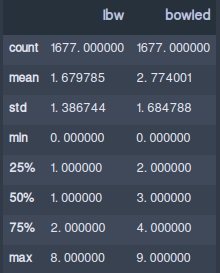
\includegraphics[width=0.25\textwidth]{lbwbowled.png}
    \caption{Statistical analysis for data for first hypothesis.}
    \label{fig:eleven}
  \end{figure}

  The first null hypothesis is rejected as the p value is less than the significance value. Figure ~\ref{fig:twelve}
  \begin{figure}[!htb]
      \centering
      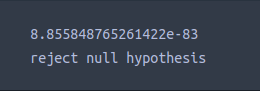
\includegraphics[width=0.25\textwidth]{lbwbowledhypo.png}
      \caption{First hypothesis result.}
      \label{fig:twelve}
    \end{figure}


\item
\begin{itemize}
    \item H(0):Wickets fallen in the first 70\% of the first innings is equal to the wickets fallen in the last 30\% of the first innings
    \item H(A):Wickets fallen in the first 70\% of the first innings is not equal to the wickets fallen in the last 30\% of the first innings
\end{itemize}
The second null hypothesis is rejected as the p value is less than the significance value. Figure ~\ref{fig:thirteen}
\begin{figure}[!htb]
    \centering
    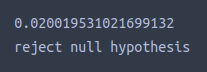
\includegraphics[width=0.25\textwidth]{secondone.png}
    \caption{Second hypothesis result}
    \label{fig:thirteen}
  \end{figure}

\item
\begin{itemize}
    \item H(0):Wickets fallen in the first 71\% of the first innings is equal to the wickets fallen in the last 29\% of the first innings
    \item H(A):Wickets fallen in the first 71\% of the first innings is not equal to the wickets fallen in the last 29\% of the first innings
\end{itemize}
The third null hypothesis is accepted as the p value is greater than the significance value. Figure ~\ref{fig:fourteen}
\begin{figure}[!htb]
    \centering
    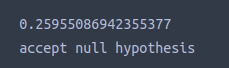
\includegraphics[width=0.25\textwidth]{secondsecond.png}
    \caption{Third hypothesis result}
    \label{fig:fourteen}
  \end{figure}

\item
\begin{itemize}
    \item H(0):Wickets fallen in the first 50\% of the first innings is equal to the wickets fallen in the last 50\% of the first innings
    \item H(A):Wickets fallen in the first 50\% of the first innings is not equal to the wickets fallen in the last 50\% of the first innings
\end{itemize}
The fourth null hypothesis is rejected as the p value is less than the significance value. Figure ~\ref{fig:fifteen}
\begin{figure}[!htb]
    \centering
    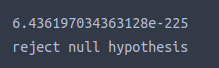
\includegraphics[width=0.25\textwidth]{secondthird.png}
    \caption{Fourth hypothesis result}
    \label{fig:fifteen}
  \end{figure}

\item
\begin{itemize}
    \item H(0):Wickets fallen in the first 10 overs of the first innings is equal to the wickets fallen in the last 10 overs of the first innings
    \item H(A):Wickets fallen in the first 10 overs of the first innings is not equal to the wickets fallen in the last 10 overs of the first innings
\end{itemize}

The fifth null hypothesis is rejected as the p value is less than the significance value. Figure ~\ref{fig:sixteen}
\begin{figure}[!htb]
    \centering
    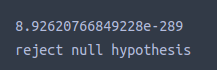
\includegraphics[width=0.25\textwidth]{secondfourth.png}
    \caption{Fifth hypothesis result}
    \label{fig:sixteen}
  \end{figure}

  The data for the second, third, fourth and fifth hypothesis lead to following statistics: Figure ~\ref{fig:seventeen}
\begin{figure}[!htb]
    \centering
    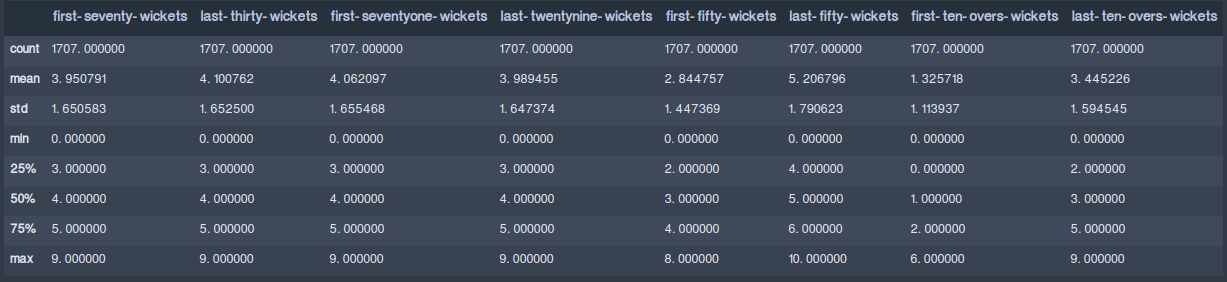
\includegraphics[width=0.5\textwidth]{second.png}
    \caption{Statistical analysis for data for second, third, fourth and fifth hypothesis.}
    \label{fig:seventeen}
  \end{figure}

\item
\begin{itemize}
    \item H(0):There is an equal probability of wicket by the first category of dismissal and second category of dismissal
    \item H(A):There is an equal probability of wicket by the first category of dismissal and second category of dismissal
\end{itemize}
 
The data for the sixth hypothesis lead to following statistics: Figure ~\ref{fig:eighteen}
  
\begin{figure}[!htb]
    \centering
    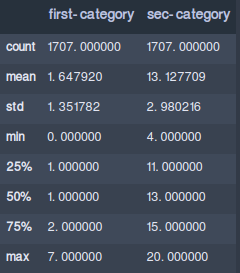
\includegraphics[width=0.25\textwidth]{third.png}
    \caption{Statistical analysis for data for sixth hypothesis.}
    \label{fig:eighteen}
  \end{figure}

  The sixth null hypothesis is rejected as the p value is less than the significance value. Figure ~\ref{fig:ninteen}
  \begin{figure}[!htb]
    \centering
    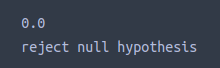
\includegraphics[width=0.25\textwidth]{thirdone.png}
    \caption{Sixth hypothesis result}
    \label{fig:ninteen}
  \end{figure}

\end{enumerate}
The level of significance for the hypothesis have been set to 5\%.
The above hypothesis have been tested using statistics.\newline
For first hypothesis the batsman dismissed by lbw and bowled in the provided matches have been conted and 
then the values in both the methods have been compared using paired t-test statistical model.\newline
For second hypothesis first the 70\% overs have been calculated and then the number of dismissals have been calculated.
These wickets have been then compared to the number of wickets that have fallen in the last 30\% overs of the match.\newline
The same procedure have been followed for the third, fourth and the fifth hypothesis.\newline
In the last hypothesis the dismissal method have been divided into the following two categories:
    \begin{itemize}
        \item first category =['run out','hit wicket','obstructing the field','retired out','stumped']
        \item Second category= ['caught','bowled','lbw','caught and bowled']
    \end{itemize}
then the number of wickets for each category have been calculated and compared using paired t-test. 
\subsection{Machine Learning Model}
Machine learning model has been created for the data of Virat Kohli. The runs scored by him has been predicted.
The correlation matrix for the scorecard is shown in Figure ~\ref{fig:twenty}. According to which the runs scored by Virat Kohli
majorly depends on the number of balls he faced and the runs he scored on these balls.
\begin{figure}[!htb]
    \centering
    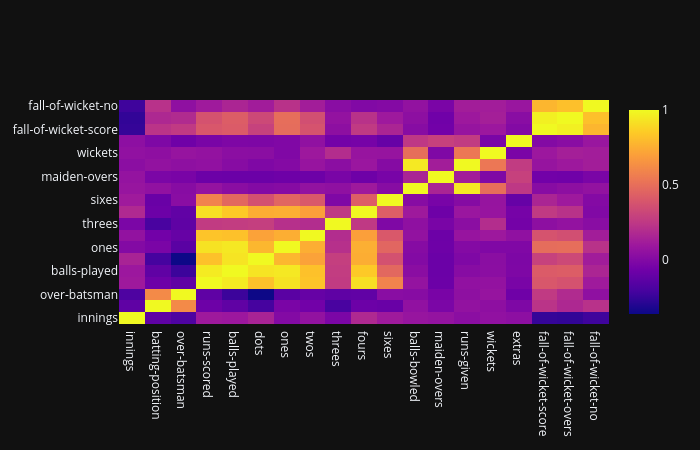
\includegraphics[width=0.5\textwidth]{correlation.png}
    \caption{Correlation matrix of the scorecard for Virat Kohli}
    \label{fig:twenty}
  \end{figure}
The balls he played has been used to predict the runs he will score using Linear Regression.
\section{Result and Discussion}
After performing the statistical analysis we can suggest following:
\begin{itemize}
    \item The mean wickets fallen in the first 71\% overs (that translates to 35.3 overs) is equal to the mean wickets fallen in the rest of the first inning (i.e. 24.3 overs).
\end{itemize}
\section{Future Work}
This cricket analysis can be further extended by analyzing data more closely and generating player wise insights. Also machine learing models can
be created using this dataset. It can be further extended to find the attributes that contribute to the result obtained of the statistical analysis.
\appendix
\section{Information of Dataset}
The dataset comprises of two files, one file comprises of each ODI match description and the other file has the scorecard of every ODI match. These matches can be uniquely
identified using match id. Attributes in both the files are as follows:
\begin{itemize}
\item Scorecard:
\begin{enumerate}
    \item match-id: Unique id of each match, that can uniquely identify a match between scorecard and match information file.
    \item innings: Innings number (Can be 0 or 1)
    \item name: Name of the player
    \item batting-position: Batting position of the player (0 if the player didn't bat)
    \item over-batsman: Over at which said batsman came out to play
    \item runs-scored: Runs scored by the player
    \item balls-played: Number of balls played by the player as a batsman.
    \item dots: Number of dot balls played by the player.
    \item ones: Number of balls when the player scored a single run.
    \item twos: Number of balls when the player scored two runs.
    \item threes: Number of balls when the player scored three runs.
    \item fours: Number of balls when the player scored four runs.
    \item sixes: Number of balls when the player scored six runs.
    \item wicket-method: Dismissal method of the player (0 if player remained not out or didn't come out to bat)
    \item balls-bowled: Number of balls that the player bowled as a bowler (0 if the player didn't bowled at all)
    \item maiden-overs: Number of overs in which the player didn't give a single run as a bowler.
    \item runs-given: Number of runs that the batsman scored on the said player's balls 
    \item wickets: Wickets taken by the player 
    \item extras: Extras given by the player as a bowler.
    \item fall-of-wicket-score: Score at which the player got out.
    \item fall-of-wicket-over: Over at which the player got out.
    \item fall-of-wicket-no: Wicket number at which the player got out.
    \item fall-of-wicket-bowler: Bowler who got the wicket (0 in case of run out).
\end{enumerate}
\item Match Information:
\begin{enumerate}
    \item city: City in which match was held
    \item competition: Competition name
    \item date: Date of match
    \item match-id: Unique id of each match, that can uniquely identify a match between scorecard and match information file.
    \item gender: Gender of the teams playing the match. (Either male or female)
    \item match-number: Number of the match in the respective series or competition
    \item match-referee: Match refree name
    \item method: D/L if match ended by D/L rule
    \item neutralvenue: true or false based upon the home venue of both the teams
    \item outcome: (No result or tie), if none of the two team win the match
    \item player-of-match: Name of the player of the match
    \item reserve-umpire: Name of reserved umpire of the match
    \item season: Year in which match was played
    \item series: Series name of which the match was a part
    \item team-0: First team name
    \item team-1: Second team name
    \item toss-decision: (Fielding or batting) Toss decision by toss winner team
    \item toss-winner: Toss winner team name
    \item tv-umpire: TV umpire name
    \item umpire-0: First umpire name
    \item umpire-1: Second umpire name
    \item venue: Ground name where match is being held
    \item winner: Winner of the match
    \item winner-runs: Winner score difference
    \item winner-wickets: Winner wicket difference
\end{enumerate}
\end{itemize}
\section{Source Code of Implementation}
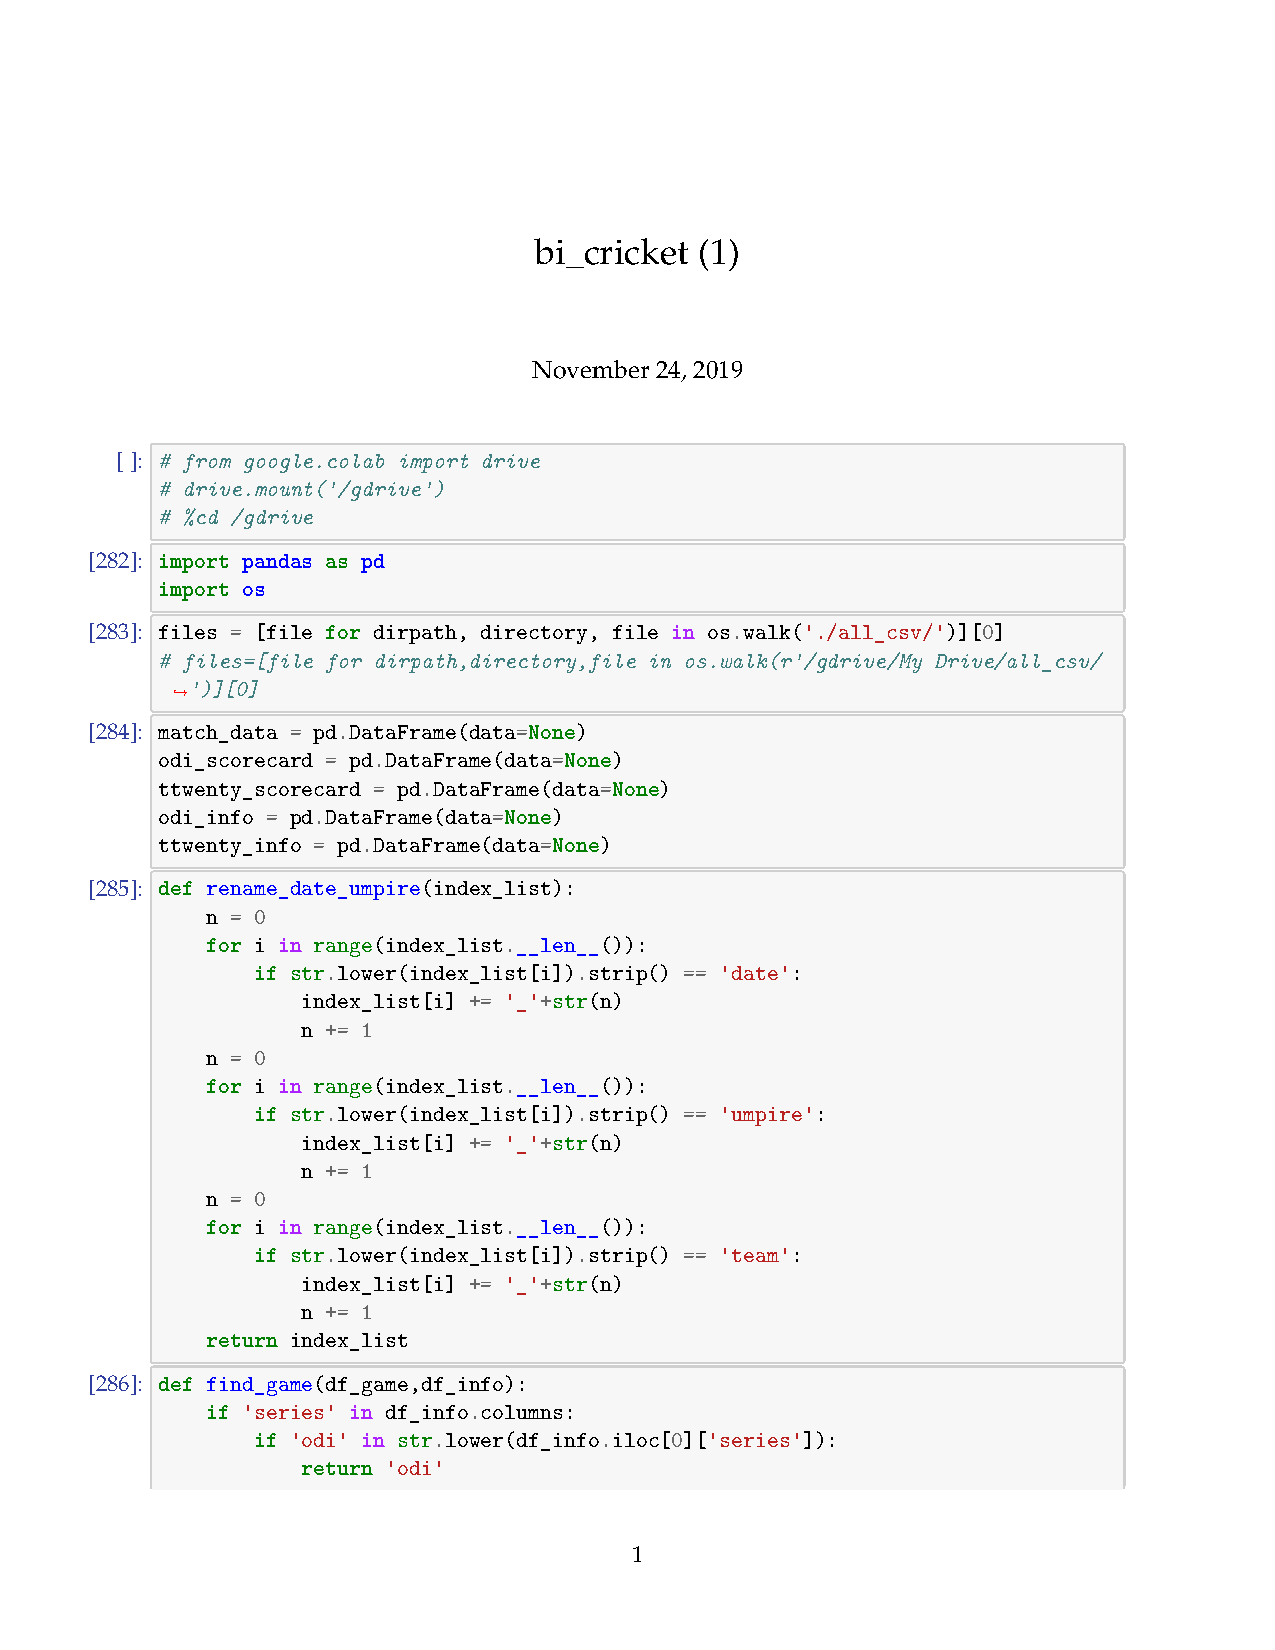
\includepdf[pages=-]{bicricket.pdf}
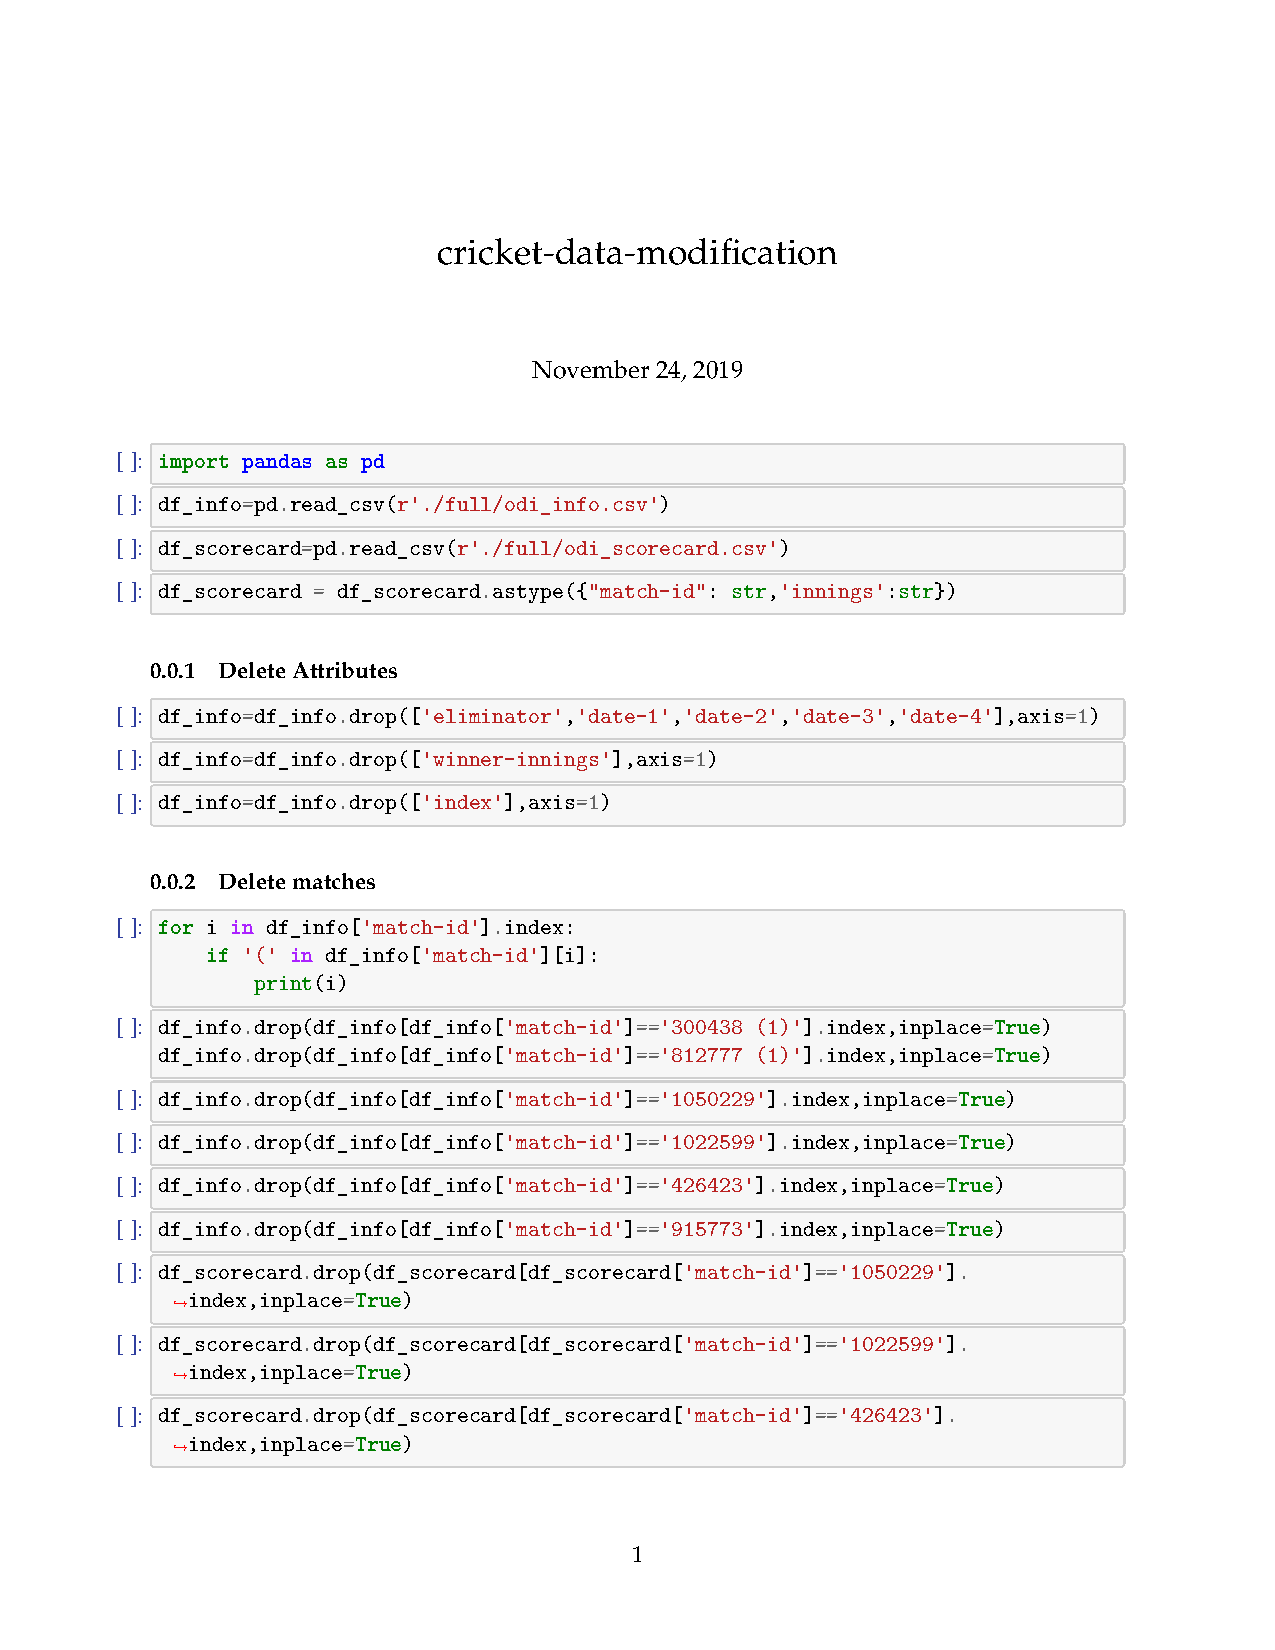
\includepdf[pages=-]{cricketdatamodification.pdf}
The interactive visualizations cannot be shown in LaTex therefore, here is the link for all the Jupyter notebook: \href{https://nbviewer.jupyter.org/github/dev-SB/cricket-bi/blob/master/vis-cricket.ipynb}{vis-cricket.ipynb}.
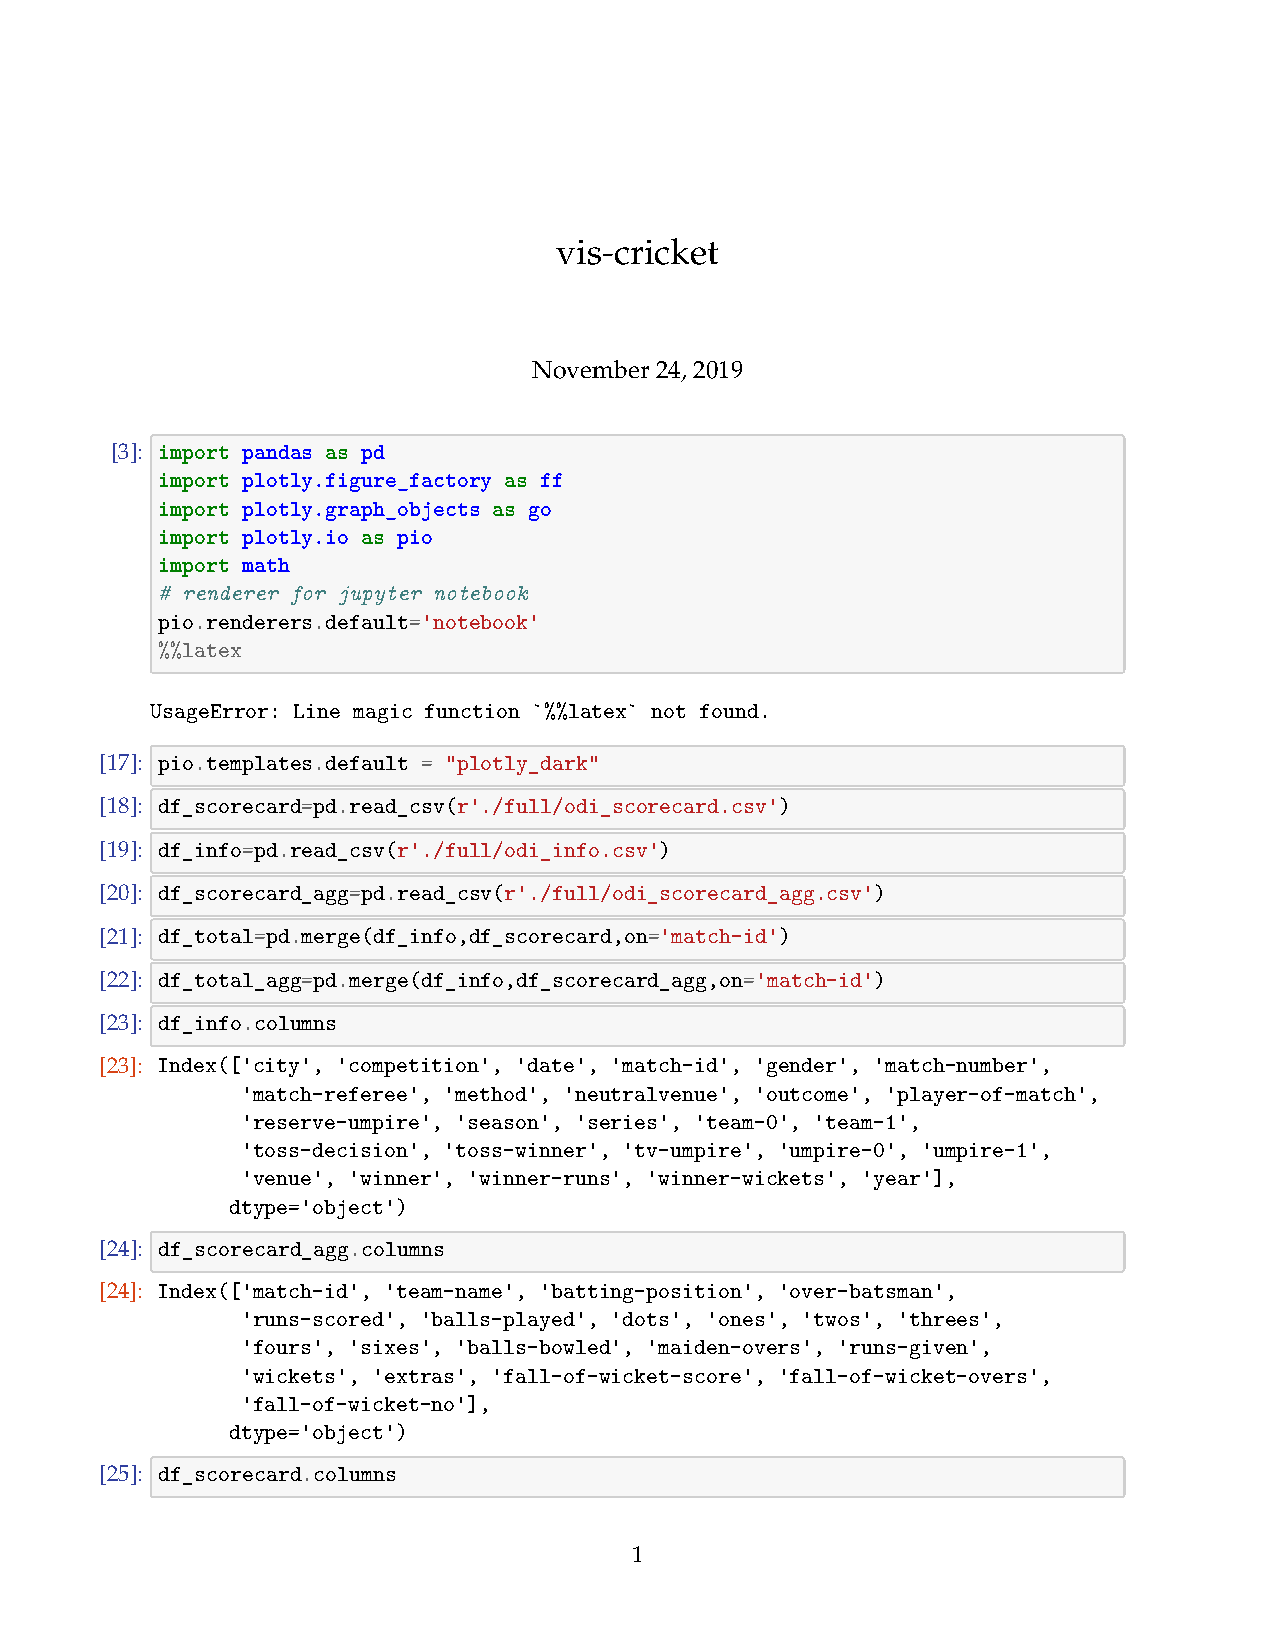
\includepdf[pages=-]{viscricket.pdf}
The interactive visualizations cannot be shown in LaTex therefore, here is the link for all the Jupyter notebook: \href{https://nbviewer.jupyter.org/github/dev-SB/cricket-bi/blob/master/hypothesis.ipynb}{hypothesis.ipynb}.
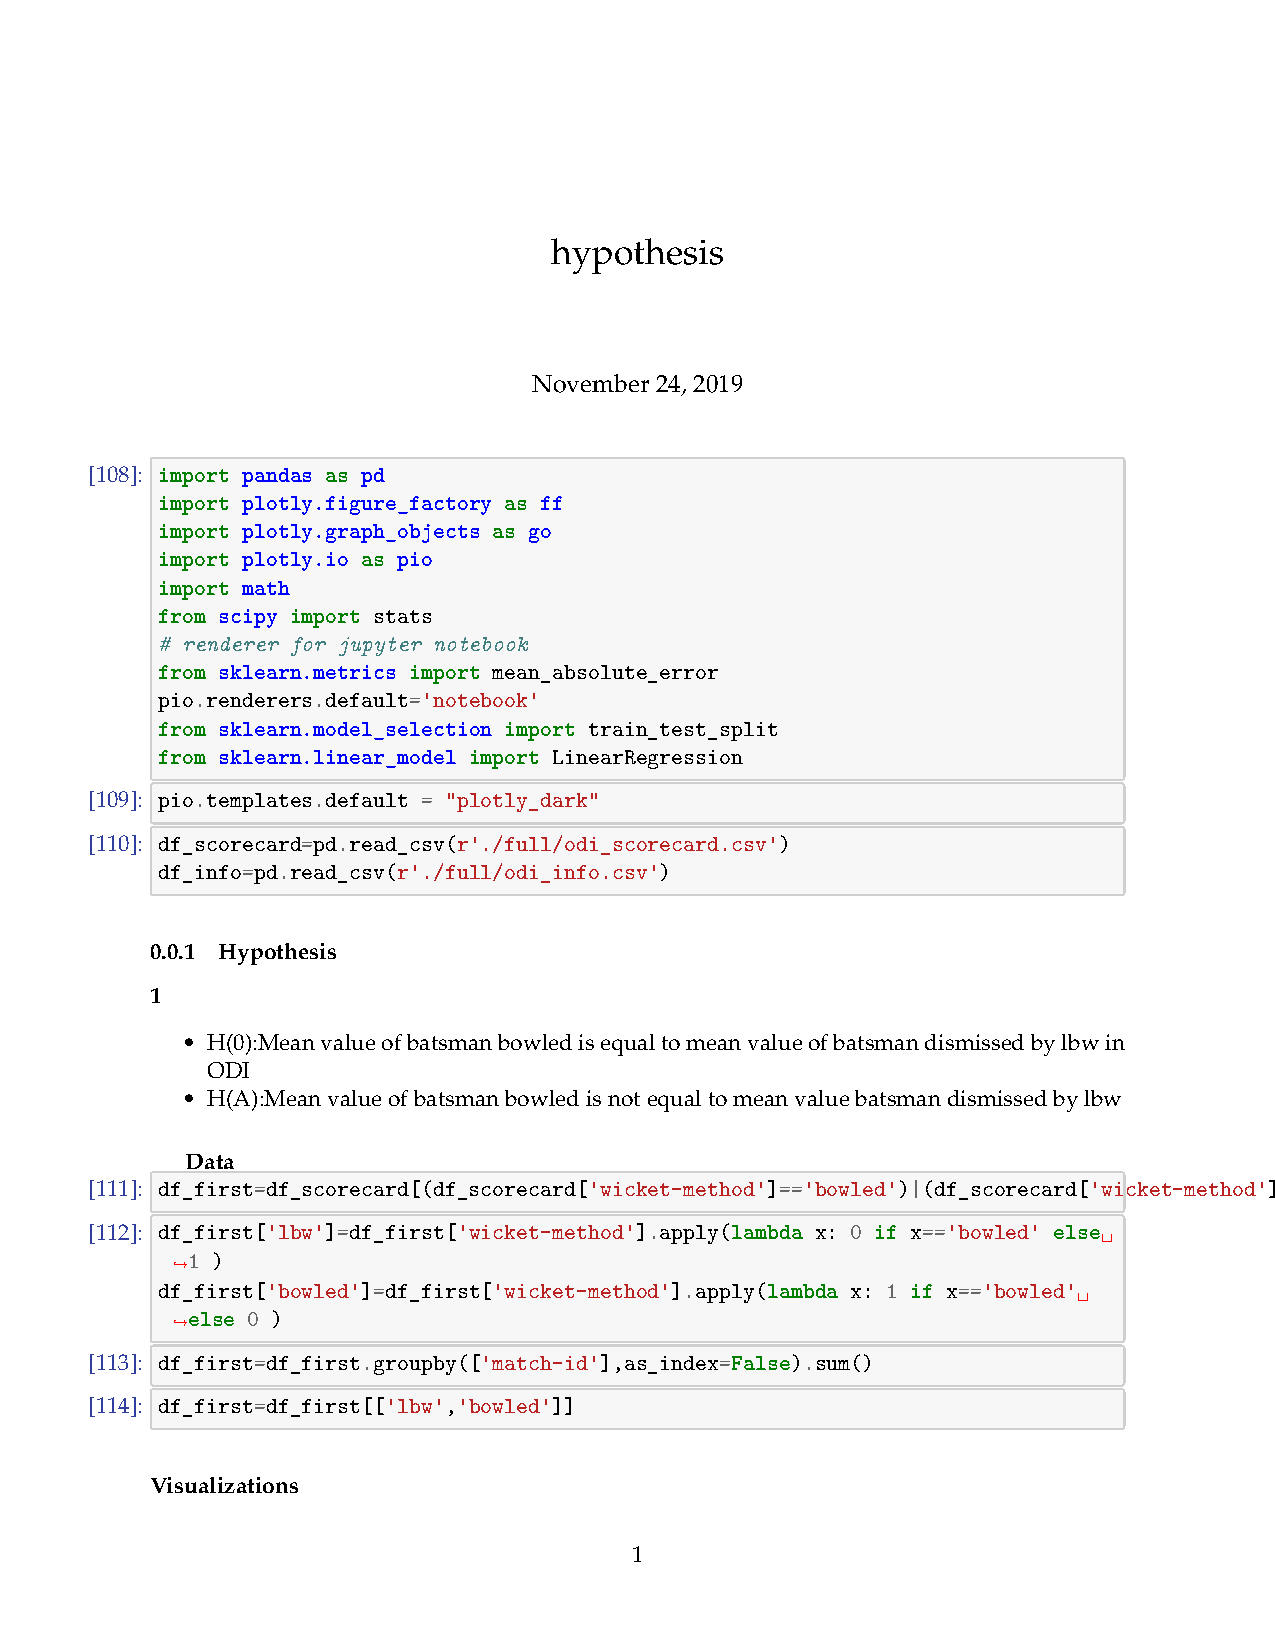
\includepdf[pages=-]{hypothesisnb.pdf}
\end{document}